\documentclass[11pt]{article}
\usepackage[utf8]{inputenc}
%\usepackage[T1]{fontenc}
\usepackage{amssymb}
\usepackage{amsmath}
\usepackage{enumerate}
\usepackage{fullpage}
\usepackage{polski}  
\usepackage{indentfirst} 
\usepackage[pdftex]{graphicx}
\usepackage{multirow}
\usepackage{placeins}
\usepackage{multicol}
\usepackage{textcomp}

\author{Łukasz Dubiel}

\begin{document}

\section{Opracowywanie wyników}
\begin{multicols}{2}

Wyniki dla prądu stałego
\begin{center}

\begin{tabular}{|r|r|}
\hline
	U[V] & I[A] \\
\hline
	0 & 0\\
	1,22 & 0,039\\
	2,24 & 0,072\\
	3,06 & 0,099\\
	4,91 & 0,159\\
	7,70 & 0,249\\
	9,17 & 0,296\\
	11,68 & 0,374\\
	8,06 & 0,259\\
	5,81 & 0,186\\
	4,54 & 0,146\\
	3,20 & 0,103\\
	2,13 & 0,068\\
	1,31 & 0,042\\
\hline
\end{tabular}
\end{center}

$$ I = U G $$
$$ G = \frac{I}{U} $$
Korzystając z metody najmniejszych kwadratów dla pomiarów uzyskujemy 
$$ G = 0.03214\ S $$
$$ \Delta G = 6 \cdot 10^{-5}\ S $$
$$ R = \frac{1}{G} = 31.1\ \Omega $$
$$ \Delta R = \left| \frac{\partial R}{\partial G} \right| \Delta G = \frac{1}{G^2} \Delta G = 0,06\  \Omega $$

\end{multicols}

\begin{multicols}{2}

Wyniki dla prądu przemiennego

\begin{center}
\begin{tabular}{|r|r|}
\hline
	U[V] & I[A] \\
\hline
	0,92 & 0,0021\\
	3,13 & 0,0062\\
	4,70 & 0,0086\\
	7,08 & 0,0119\\
	8,72 & 0,0139\\
	11,42 & 0,0171\\
	13,01 & 0,0189\\
	14,36 & 0,0202\\
	10,72 & 0,0163\\
	7,51 & 0,0124\\
	5,05 & 0,0091\\
	2,30 & 0,0048\\
	1.13 & 0,0026\\
\hline
\end{tabular}
\end{center}
\columnbreak
$$ I = Y U $$
$$ Y = \frac{I}{U}$$
$$ Y = 0.00138 \ S $$
$$ \Delta Y = 4 \cdot 10^{-5}\ S $$
$$ Z = \frac{1}{Y} = 723.5115\ \Omega $$
$$ \Delta Z = \left| \frac{\partial Z}{\partial Y} \right| \Delta Y = \frac{1}{Y^2}\Delta Y = 26\ \Omega$$
\end{multicols}
$$ Z = R + \omega L $$
$$ L = \frac{Z - R}{2 \pi f} = \frac{723 - 31.1}{2 \cdot 3,14 \cdot 50} = 2,2\ H $$
$$ \Delta L = \left| \frac{\partial{L}}{\partial{Z}} \right| \Delta Z  + \left| \frac{\partial{L}}{\partial{R}} \right| \Delta R = \frac{1}{2 \pi f}\left[|1-R|\Delta Z + |Z - 1|\Delta R \right] $$
$$ \Delta L = \frac{1}{2 \cdot 3,14 \cdot 50} (|1 - 31.1|\cdot 26 + |723-1|\cdot 0,06) = \frac{826}{314} = 2,6\ H$$

$$ \tan{d} = \frac{\omega L}{R} = 21,9 \quad
d = 87.39^o $$

\newpage
\begin{center}


\resizebox{9cm}{!}{
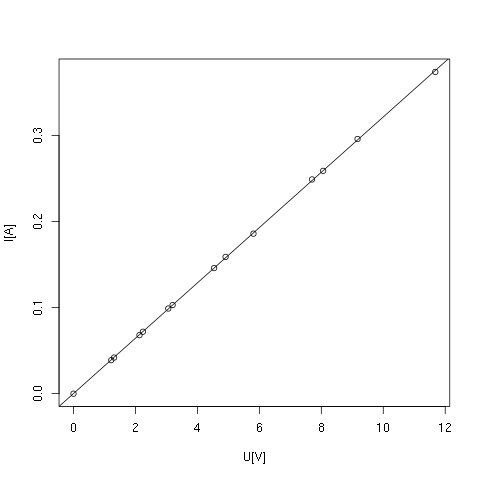
\includegraphics{wykresDC.png}}

Prąd stały

\resizebox{9cm}{!}{
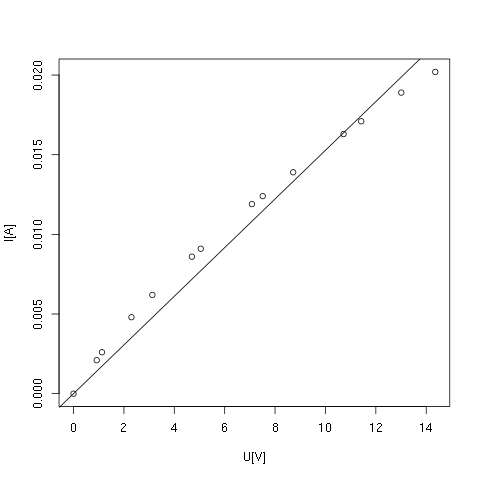
\includegraphics{wykresAC.png}}

Prąd zmienny
\end{center}
\end{document}
